\section{System Assembly}

\subsection{Basic Example}
    
\begin{frame}%[<+->]
  \frametitle{System Assembly}
  \begin{itemize}
  \item {For simplicity we will focus on the weighted
    residual statement arising from the Poisson equation,
    with $\partial \Omega_N = \emptyset$, 
    \begin{eqnarray}
      \nonumber
      (\R( u^h ), v^h) := \hspace{2.5in} \\  \nonumber
      \int_{\Omega^h}  \left[ \nabla u^h \cdot \nabla v^h - fv^h \right] dx %\\ \nonumber
      %+ \int_{\partial \Omega^h_N} u_N v^h \;ds
      =0 \hspace{.5in} \forall v^{h} \in \mathcal{V}^{h}
    \end{eqnarray}
  }
  \end{itemize}
\end{frame}


    
\commentout{
\begin{frame}%[c]
%  \frametitle{Poisson Equation}
  \begin{itemize}    
  \item{
%%     \only<1>
%% 	{
	  The integral over $\Omega^h$ \ldots
%%	}
	  \visible<2->
	  {
	    is written as
	    a sum of integrals over the $\alert{N_e}$ finite elements: % $\Omega_e^h$
	  }
  }
  \end{itemize}
	  
  %\begin{block}{}
    \begin{eqnarray}
	\nonumber
	%(\R( u^h ), v^h) &:=& %\hspace{3in} \\  \nonumber
	0 &=&
	\phantom{\sum_{e=1}^{N_e}}
	\int_{\Omega^h}  \left[ \nabla u^h \cdot \nabla v^h - fv^h \right] dx
	\hspace{.2in} \forall v^{h} \in \mathcal{V}^{h}
	\\ \nonumber
	\visible<2>
	    {
	&=&\alert{\sum_{e=1}^{N_e}}
	      \int_{\alert{\Omega_e}}
	      \left[ \nabla u^h \cdot \nabla v^h - fv^h \right] dx
	      \hspace{.2in} \forall v^{h} \in \mathcal{V}^{h}
	      \\ \nonumber
	    }
%% 	    \visible<3>
%% 		{
%% 	&=&\alert{\sum_{e=1}^{N_e}}
%% 	      \underbrace{\int_{\alert{\Omega_e}}
%% 	      \left[ \nabla u^h \cdot \nabla v^h - fv^h \right] dx}_{\text{We must compute this}}
%% 	      \hspace{.2in} \forall v^{h} \in \mathcal{V}^{h}
%% 		}
      \end{eqnarray}
    %\end{block}
%%     \begin{eqnarray}
%%       \nonumber
%%       (\R( u^h ), v^h) &=& \int_{\Omega^h} (\ldots) \\
%%       \nonumber
%%       &=& \sum_{e=1}^{N_e} \int_{\Omega_e}(\ldots)\hspace{.25in} \forall v^{h} \in \mathcal{V}^{h}
%%     \end{eqnarray}
    
%  \item{The $v^h$ typically have support over only a small subset of the elements.}
\end{frame}
}


    
\commentout{
\begin{frame}
  % \frametitle{Weighted Residual Statement}
    \begin{columns}[t]
    \column{.5\textwidth}
    \begin{block}{}
%%       \only<1>
%%       {
%% 	To node $i$ we associate a basis function $\psi_i$ such that for any $v^h \in \mathcal{V}^h$
%% 	we have
%% 	\begin{equation}
%% 	  \nonumber
%% 	  v^h = \sum_{i=1}^{N_n} c_i \psi_i
%% 	\end{equation}
%% 	for some constants $c_i$.
%%       }

%%       \only<2>
%%       {
%% 	\begin{itemize}
%% 	  \item{The $\psi_i$ are non-zero only over the elements adjacent to node $i$.}
%% 	  \item{For example, $\psi_i$ could be the linear ``hat'' function.
%% 	    %with value 1
%% 	    %at node $i$ and zero at all other nodes.
%% 	  }
%% 	\end{itemize}
%%       }

%%       \only<3->
%%       {
	\begin{itemize}
	  \item{An element integral will have contributions only
	    from the global basis functions corresponding to its nodes.}
	  \item{We call these local basis functions $\phi_i$, $0 \leq i \leq N_s$.}
	\end{itemize}
%%      }
    \end{block}

%%       \visible<3->
%%       {
	    \begin{equation}
	      \nonumber
	      \left. v^h \right|_{\Omega_e} = \sum_{i=1}^{N_s} c_i \phi_i
	    \end{equation}
%%      }
      \visible<2>
      {
	    \begin{equation}
	      \nonumber
	      \alert{\int_{\Omega_e}} v^h \;\alert{dx}
	      = \sum_{i=1}^{N_s} c_i \alert{\int_{\Omega_e}}\phi_i \;\alert{dx}
	    \end{equation}

      }
%}
%  \end{itemize}
    \column{.5\textwidth}
    %\begin{block}{}
      \begin{center}
%% 	\only<1>
%% 	    {
%% 	      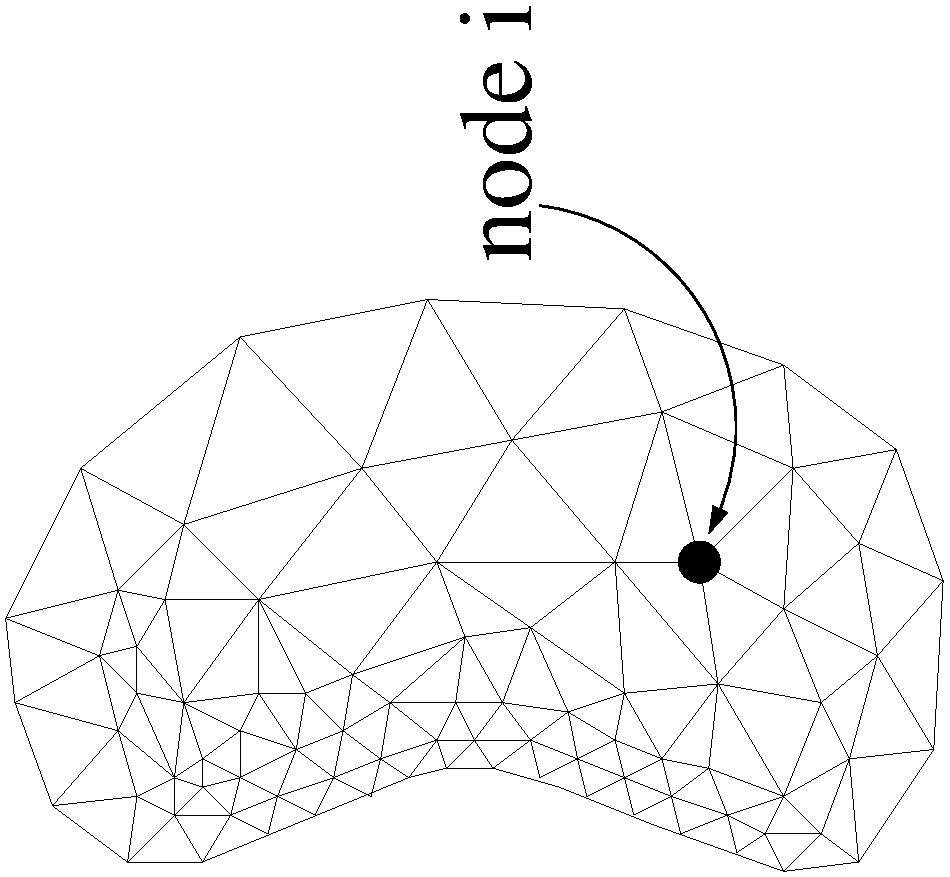
\includegraphics[width=2in]{figs/node_i}
%% 	    }
%% 	\only<2>
%% 	    {
%% 	      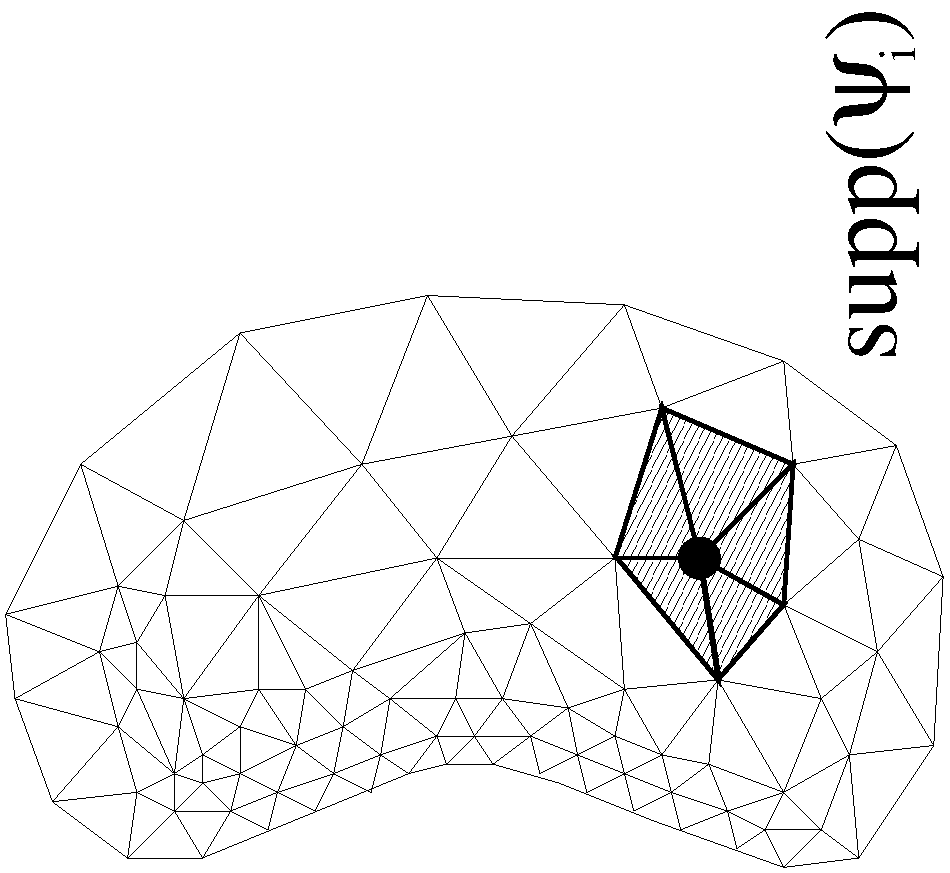
\includegraphics[width=2in]{figs/phi_i}
%% 	    }
%% 	\only<3->
%% 	    {
	      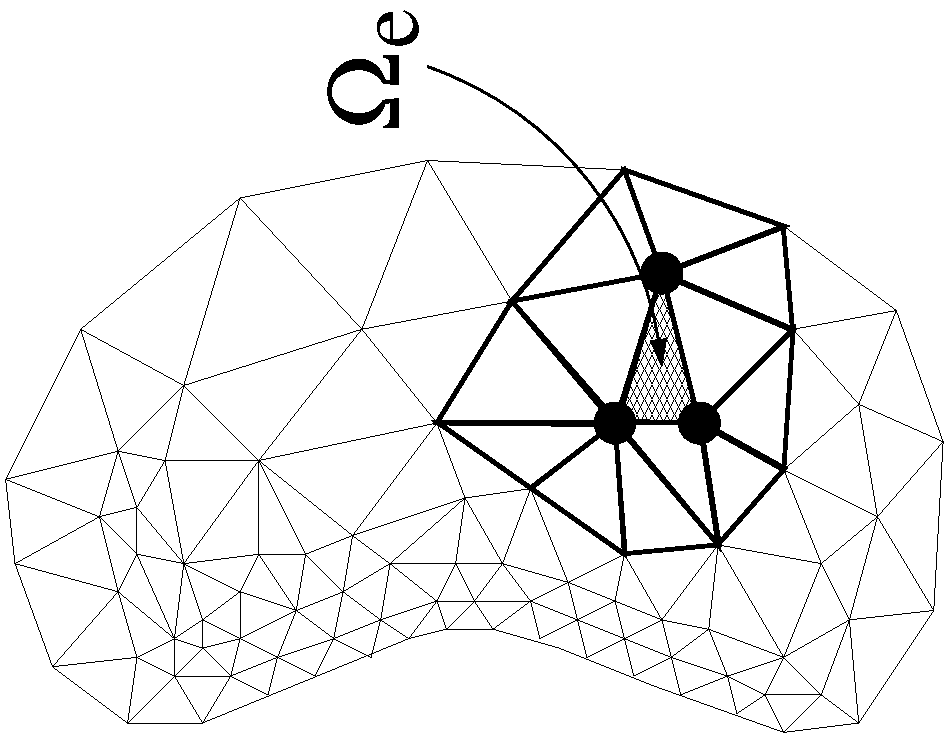
\includegraphics[width=2in]{figs/phi_ijk}
%%	    }
      \end{center}
    \end{columns}
\end{frame}
}



%% \frame%[t]
%%     {
%%   \frametitle{Poisson Equation}
%%   \begin{itemize}    
%%   \item
%%     {
%%       \visible<1->
%%       {
%% 	The element integrals \ldots
%%       }
%%       \visible<2->
%%       {
%% 	are written in terms of the local ``$\alert<2>{\phi_i}$'' basis functions \ldots
%%       }
%%       \visible<3>
%%       {
%% 	which can be expressed naturally in matrix notation.
%% 	%element ``stiffness matrix'' $\alert{\bv{K_e}}$
%% 	%and ``load vector'' $\alert{\bv{F_e}}$. 
%%       }
%%     }
%%   \end{itemize}
%%     \begin{eqnarray}
%%       %\begin{center}
%% 	\nonumber
%% 	%\begin{array}{c}
%% 	\int_{\Omega_e} \left[ \nabla u^h \cdot \nabla v^h - fv^h \right] dx
%% 	\hspace{.75in} \\ \nonumber
%% 	  \visible<2->
%% 	      {
%% 		\Downarrow \hspace{1.5in} \\ \nonumber
%% 		%
%% 		\alert<2>{\sum_{j=1}^{N_s}}  \alert<2>{u_j}   \int_{\Omega_e}
%% 		\nabla \alert<2>{\phi_j} \cdot \nabla \alert<2>{\phi_i} \;dx
%% 		- \int_{\Omega_e}  f\alert<2>{\phi_i} \;dx
%% 		\hspace{.15in},\hspace{.15in} i = 1,\ldots,N_s \\ \nonumber
%% 	      }
%% 	      \visible<3>
%% 	      {\Downarrow \hspace{1.5in} \\ \nonumber
%% 		%
%% 		\bv{K_e} \bv{U_e} - \bv{F_e} \hspace{1.25in}
%% 	      }
%% 	%\end{array}
%%       %\end{center}
%%     \end{eqnarray}
%%     }



\begin{frame}%[t]
%  \frametitle{Poisson Equation}
  \begin{itemize}    
    \visible<1->
	{
	\item
	  {
	    The element integrals \ldots
	    \begin{equation}
	      \nonumber
	      \int_{\Omega_e} \left[ \nabla u^h \cdot \nabla v^h - fv^h \right] dx
	    \end{equation}
	  }
	}

	
      \visible<2->
      {
	\item{
	  are written in terms of the local ``$\alert<2>{\phi_i}$'' basis functions
	  \begin{equation}
	    \nonumber
		\alert<2>{\sum_{j=1}^{N_s}}  \alert<2>{u_j}   \int_{\Omega_e}
		\nabla \alert<2>{\phi_j} \cdot \nabla \alert<2>{\phi_i} \;dx
		- \int_{\Omega_e}  f\alert<2>{\phi_i} \;dx
		\hspace{.15in},\hspace{.15in} i = 1,\ldots,N_s
	  \end{equation}
	}
      }
      \visible<3>
      {
	\item{
	  This can be expressed naturally in matrix notation as
	\begin{equation}
	  \nonumber
	  \bv{K^e} \bv{U^e} - \bv{F^e} 
	\end{equation}
	}
      }
  \end{itemize}
 \end{frame}


\commentout{
\begin{frame}%[<+->]
  %  \frametitle{Poisson Equation}
  \begin{itemize}
    \visible<1->{
    \item{
      The entries of the element stiffness matrix are the integrals
      \begin{equation}
	\nonumber
	\bv{K}^e_{ij} := 
	\int_{\Omega_e}
	\nabla \phi_j \cdot \nabla \phi_i \;dx
      \end{equation}
    }
    }
    \visible<2->{
    \item{ While for the element right-hand side we have 
      \begin{equation}
	\nonumber
	\bv{F}^e_{i} := 
	\int_{\Omega_e} f \phi_i \;dx
      \end{equation}
    }
    }
    \visible<3>{
    \item{ The element stiffness matrices and right-hand sides can be ``assembled'' to 
      obtain the global system of equations
      \begin{equation}
	\nonumber
	\bv{K} \bv{U} = \bv{F}
      \end{equation}    
    }
    }
  \end{itemize}
\end{frame}
}






\begin{frame}[t]
%  \frametitle{Poisson Equation}
  \begin{block}{}
    \begin{itemize}    
  \item{
    The integrals are performed on a ``reference'' element $\alert<1>{\hat{\Omega}_e}$, transformed via Lagrange basis to the geometric element.
    }
  \end{itemize}
  \end{block}\vspace{-.3in}
  \begin{center}
  \begin{tabular}{lll} \\ 
    %\fbox{
      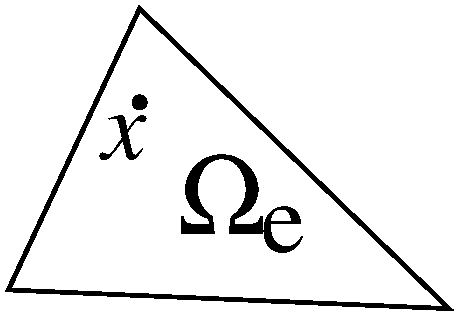
\includegraphics[width=.5in,angle=-90]{figs/physical_element}
    %}
       &
  \only<1,3->
  {
       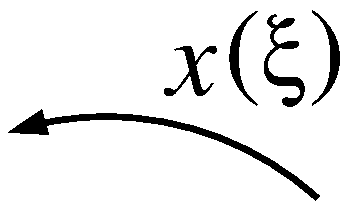
\includegraphics[height=.5in,angle=-90]{figs/map}
  }
  \only<2>
  {
       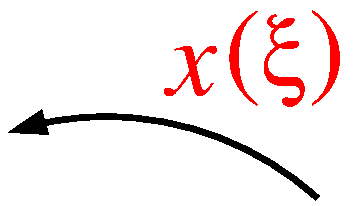
\includegraphics[height=.5in,angle=-90]{figs/map_red}
  }
       &
  \only<1>
  {
       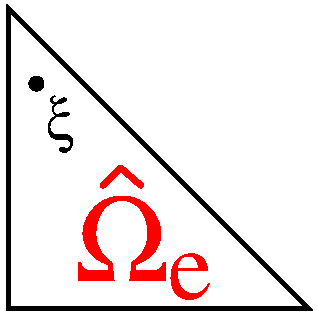
\includegraphics[width=.7in,angle=-90]{figs/reference_element_red}
       }
  \only<2->
  {
       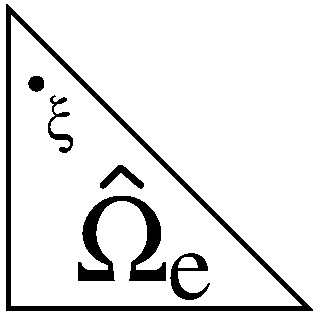
\includegraphics[width=.7in,angle=-90]{figs/reference_element}
       }
     \end{tabular}
  \end{center}


  \only<2>
      {
	\begin{block}{}
	\begin{itemize}    
	\item{
	  The Jacobian of the map $\alert{x(\xi)}$ is $\alert{J}$.
	}
	\end{itemize}
	\end{block}
	\begin{equation}
	  \nonumber
	  \bv{F}^e_{i} = \int_{\Omega_e} f \phi_i dx
	  =  \int_{\alert{\hat{\Omega}_e}}
	  f (\alert{x(\xi)}) \phi_i \alert{|J|} d\alert{\xi}
	\end{equation}
      }

\commentout{
\only<3>
{
  \begin{block}{}
  \begin{itemize}    
  \item{
    %The gradients are transformed
    Chain rule: 
    $\nabla 
    = J^{-1}\nabla_{\!\xi}
    := \alert{\hat{\nabla}_{\!\xi}}$.
  }
  \end{itemize}
  \end{block}
  \begin{equation}
    \nonumber
    \bv{K}^e_{ij} =
    \int_{\Omega_e}
    \nabla \phi_j \cdot \nabla \phi_i \;dx =
    \int_{\hat{\Omega}_e}
    \alert{\hat{\nabla}_{\!\xi}} \phi_j \cdot
    \alert{\hat{\nabla}_{\!\xi}} \phi_i \;|J| d\xi
  \end{equation}
}
}
\end{frame}





    
\begin{frame}[t]
%	\frametitle{Poisson Equation}
	\begin{block}{}
	\begin{itemize}    
	\item{
	  The integrals on the ``reference'' element are approximated via numerical
	  quadrature.
	}
	  \visible<2->
	      {
	      \item{The quadrature rule has $\alert{N_q}$ points
		``$\alert{\xi_q}$'' and weights ``$\alert{w_q}$''.}
	      }
	\end{itemize}
	\end{block}
\only<3>
{
	\begin{eqnarray}
	  \nonumber
%	  \only<3-4>
%	      {
		\bv{F}^e_{i} &=&
		\int_{\hat{\Omega}_e} f \phi_i |J| d\xi
		\\ \nonumber
%	      }
%	      \only<4>
%		  {
		    &\approx&
		    \alert{\sum_{q=1}^{N_q}}
		    f(x(\alert{\xi_q})) \phi_i(\alert{\xi_q})
		    |J(\alert{\xi_q})| \alert{w_q}
%		  }
	\end{eqnarray}
}

\only<4>
{
	\begin{eqnarray}
	  \nonumber
%	  \only<5-6>
%	      {
		\bv{K}^e_{ij} &=&
		\int_{\hat{\Omega}_e}
		\nabla \phi_j \cdot
		\nabla \phi_i \;|J| d\xi
		\\ \nonumber
%	      }
%	      \only<6>
%		  {
		    &\approx&
		    \alert{\sum_{q=1}^{N_q}}
		    \nabla \phi_j(\alert{\xi_q}) \cdot
		    \nabla \phi_i(\alert{\xi_q})
		    |J(\alert{\xi_q})| \alert{w_q}
%		  }
	\end{eqnarray}
}
\end{frame}
    

\begin{frame}[t]
%	\frametitle{Poisson Equation}
	\begin{block}{}
	At the $q$th quadrature point, \texttt{LibMesh} can provide
variables including:
	
%% 	\item{``\texttt{JxW[q]}'' = $|J(\xi_q)| w_q$
%% 	  %the scalar value of the element Jacobian map times
%% 	  %the quadrature rule weight
%% 	}
	\end{block}
	
	\begin{center}
	  \renewcommand{\arraystretch}{1.3}
	\begin{tabular}{|l|l|l|} \hline
	  \textbf{Code} & \textbf{Math} & \textbf{Description} \\ \hline
	  \texttt{JxW[q]}
	  & $|J(\xi_q)| w_q$
	  & Jacobian times weight
	  \\ \hline
	  \texttt{phi[i][q]}
	  & $\phi_i(\xi_{q})$
	  & value of $i^{th}$ shape fn.\
	  \\ \hline
	  \texttt{dphi[i][q]}
	  & $\nabla \phi_i (\xi_q)$
	  & value of $i^{th}$ shape fn.\ gradient
	  \\ \hline
	  \texttt{d2phi[i][q]}
	  & $\nabla \nabla \phi_i (\xi_q)$
	  & value of $i^{th}$ shape fn.\ Hessian
	  \\ \hline
	  \texttt{xyz[q]}
	  & $x(\xi_q)$
	  & location of $\xi_q$ in physical space
	  \\ \hline
	  \texttt{normals[q]}
	  & $\vec{n}(x(\xi_q))$
	  & normal vector at $x$ on a side
	  \\ \hline
	  \end{tabular}
	\end{center}
	  
%      } %end frame
\end{frame}


      
\begin{frame}[fragile,t]  
%  \frametitle{Poisson Equation}
	\begin{block}{}
	  \begin{itemize}    
	  \item{ The \texttt{LibMesh} representation of the matrix and
	    rhs assembly is similar to the mathematical statements.
	  }
	  \end{itemize}
	\end{block}
\small
\begin{semiverbatim}
for (q=0; q<Nq; ++q) 
  for (i=0; i<Ns; ++i) \{
    \alert<2>{Fe(i)   += \alert<3>{JxW[q]}*\alert<4>{f(xyz[q])}*\alert<5>{phi[i][q]};}
    
    for (j=0; j<Ns; ++j)
      \alert<6>{Ke(i,j) += \alert<7>{JxW[q]}*(\alert<8>{dphi[j][q]*dphi[i][q]});}
  \}
\end{semiverbatim}
\only<2-5>
{
  \begin{equation}
    \nonumber
    \bv{F}^e_{i} = 
    \sum_{q=1}^{N_q}
    \alert<4>{f(x(\xi_q))}
    \alert<5>{\phi_i(\xi_q)}
    \alert<3>{|J(\xi_q)| w_q}
  \end{equation}
}
\only<6->
{
  \begin{equation}
  \nonumber
  \bv{K}^e_{ij} =
  \sum_{q=1}^{N_q}
  \alert<8>{
    \hat{\nabla}_{\!\xi} \phi_j(\xi_q) \cdot
    \hat{\nabla}_{\!\xi} \phi_i(\xi_q)
    }
  \alert<7>{|J(\xi_q)| w_q}
  \end{equation}
}
\end{frame}
